
\documentclass[tikz,border=2pt]{standalone}
\usepackage{tikz}
\usepackage{lmodern}
\usetikzlibrary{calc,decorations.pathreplacing}

% Visual conventions follow the existing MRNC TikZ pictures: ordinary
% components use TikZ's normal 0.4pt stroke, with compact TeX labels.
\tikzset{
  nu fibre/.style={
    x=0.78cm,
    y=0.78cm,
    line width=0.4pt,
    line cap=round,
    line join=round
  },
  nu label/.style={
    font=\scriptsize,
    inner sep=1pt
  },
  nu annotation/.style={
    font=\scriptsize,
    inner sep=1pt
  },
  nu dots/.style={
    font=\small,
    inner sep=0pt
  }
}

\begin{document}
%IV-In-m (n>1)

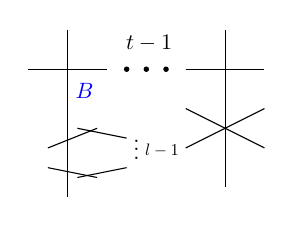
\begin{tikzpicture}[scale=0.5]
      \coordinate (1C) at (-1.50, 3.00);
  \coordinate (1D) at (-0.50, 3.00);
  \coordinate (1A) at (-1.00, 3.00);
  \coordinate (1B) at (-0.93, 3.26);

  \node[scale=0.8][above] at (1B) {$t-1$};
  \fill[black] (1C) circle (2pt);
  \fill[black] (1D) circle (2pt);
  \fill[black] (1A) circle (2pt);

      \coordinate (IVrC) at (0.00, 3.00);
  \coordinate (IVrD) at (2.00, 3.00);
  \coordinate (IVrE) at (1.00, 4.00);
  \coordinate (IVrF) at (1.00, 0.00);
  \coordinate (IVrG) at (0.00, 2.00);
  \coordinate (IVrL) at (2.00, 1.00);
  \coordinate (IVrI) at (0.00, 1.00);
  \coordinate (IVrM) at (2.00, 2.00);
  \coordinate (IVrD_1) at (1.72, 2.35);

  

  \draw (IVrC) -- (IVrD);
  \draw (IVrE) -- (IVrF);
  \draw (IVrG) -- (IVrL);
  \draw (IVrI) -- (IVrM);


 \coordinate (A) at (-4.00, 3.00);
  \coordinate (B) at (-2.00, 3.00);
  \coordinate (C) at (-3.00, 4.00);
  \coordinate (D) at (-3.00, -0.25);
  \coordinate (G) at (-2.57, 2.06);
  \coordinate (E) at (-3.50, 1.00);
  \coordinate (F) at (-2.25, 1.50);
  \coordinate (H) at (-3.50, 0.50);
  \coordinate (I) at (-2.25, 0.25);
  \coordinate (J) at (-2.75, 1.50);
  \coordinate (K) at (-1.50, 1.25);
  \coordinate (L) at (-2.75, 0.25);
  \coordinate (M) at (-1.50, 0.50);
  \coordinate (N) at (-1.25, 0.5);
  \coordinate (O) at (-0.6, 0.62);


  \draw (A) -- (B);
  \draw (C) -- (D);
  \node[scale=0.8][above, text=blue] at (G) {$B$};
  \draw (E) -- (F);
  \draw (H) -- (I);
  \draw (J) -- (K);
  \draw (L) -- (M);
  \node[scale=0.8][above] at (N) {$\vdots
$};
  \node[scale=0.6][above] at (O) {$l-1
$};
  
\end{tikzpicture}

\end{document}
